%\section{Wprowadzenie}
\section{Introduction}
%Integracja technologii baz danych z nowoczesnymi metodami
%indukcyjnego generowania wiedzy jest naturalnym kierunkiem rozwoju
%system�w bazodanowych.
The integration of the database technology with modern inductive methods of
knowledge generation is a natural direction of database systems development.
%Systemy nazywane czasem indukcyjnymi bazami
%danych potrafi� odpowiedzie� nie tylko na pytania, dla kt�rych
%odpowied� znajduje si� w bazie danych, ale r�wnie� na pytania,
%kt�re wymagaj� zsyntetyzowania i zastosowania wiedzy,
%wygenerowanej przez indukcyjne wnioskowanie z fakt�w z bazy danych
%i wcze�niejszej wiedzy~\cite{bib3}.
Systems, which are referred to as inductive data bases, allow to
finding answers to questions, to which replies are in the database
(using conventional database operators), and also to questions,
which demand synthesis of the data and knowledge generated by
induction from facts from the database and formerly gained
knowledge (using inductive operators)~\cite{bib3}.
% Schemat typowej indukcyjnej
% bazy danych przedstawiony jest na rysunku~\ref{fig:inddb}.
A schema of a typical inductive database is presented in the
Fig.~\ref{fig:inddb}.

\begin{figure}[!ht]
    \centering
        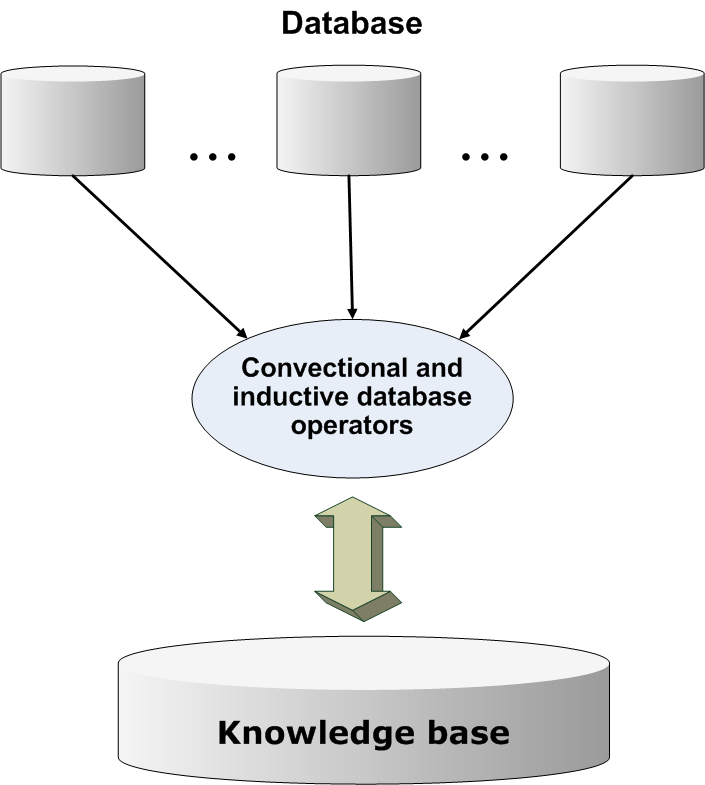
\includegraphics[width=0.6\linewidth]{img/knowledge_mining.png}
%    \caption{Indukcyjna baza danych~\cite{bib2}}
    \caption{Inductive database~\cite{bib2}}
    \label{fig:inddb}
\end{figure}
%W pierwszej cz�ci pracy przedstawione zosta�y wybrane istniej�ce
%�rodowiska wspieraj�ce uruchamianie algorytm�w uczenia maszynowego.

In this paper a component realization of the inductive database --
the \emph{Salomon} platform is proposed. Thanks to the modular
structure very good system flexibility is achieved, in comparison
to the systems described below.

This paper has the following structure. Selected machine learning
environments are described in the first part of the article.
%Dalej opisano za�o�enia, a~nast�pnie architektur� i wybrane aspekty
%implementacji komponentowej realizacji indukcyjnej bazy danych --
%platformy \emph{Salomon}.
Next the assumptions, the architecture and various implementation
aspects of \emph{Salomon} are described.
%  Dzi�ki budowie modu�owej uda�o si� uzyska�
%du�o wi�ksz� elastyczno�� systemu w stosunku do opisanych wcze�niej
%rozwi�za�.
Tests description and a case study conclude the work.
%  Ostatnia cz�� pracy prezentuje mo�liwo�ci wykorzystania
%platformy do uczenia drzew decyzyjnych.
